\chapter{Prototype Implementation}
\label{Chapter4}
\lhead{Chapter 4. \emph{Prototype Implementation}}

This chapter describes a reference implementation of the visualization methods in chapter \ref{Chapter3}.

mobile device is equipped with a camera, GPS and gyrocompass devices. The camera lets the user take video from his own point of view. GPS and gyrocompass devices give the system the position and orientation of the mobile camera, respectively.


\section{System architecture}

\subsection{Hardware}

\begin{itemize}
	\item The mobile device used is a SONY VAIO VGN-UX90PS, its specifications is in appendix \ref{AppendixA}. It has two built-in cameras. We use only the camera at the back as shown in figure \ref{fig:VAIO_Back}, at 15fps@640x480.
	\item The gyrocompass attached is an InterSense InertiaCube3. It is one of the world's smallest inertial orientation reference system, its specifications is in appendix \ref{AppendixB}. The update rate is 180Hz, which eliminates tracker induced lag. It is connected to the mobile device with and RS322-USB adapter.
	\item The RTK-GPS system is shown in Figure [cite]. It is also connected to the mobile device with and RS232-USB adapter.
\end{itemize}

\begin{figure}[htbp]
  \centering
    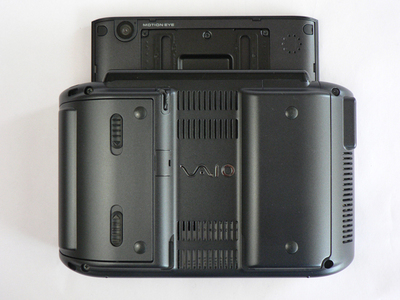
\includegraphics{./Primitives/vaio_back.jpg}
    \rule{35em}{0.5pt}
  \caption[The camera at the back of the SONY VAIO VGN-UX90PS]{The camera at the back of the SONY VAIO VGN-UX90PS}
  \label{fig:VAIO_Back}
\end{figure}

\subsection{Software}

The system does not use a server or any real surveillance camera. In place of those, 3D model of the building of the College of International Studies and the gymnasium (Figure [cite]), together with the hard coded geometry information about the virtual surveillance cameras are used.

The best visualization method is expected to be found visually and practically. A good visualization method can be the combination of many others at any extent. Thus, trial and error methodology can be applied here. To shorten the trial and error cycles, a good developmental environment of the preliminary system in this research, C language and OpenGL API \citep{Reference10} were used at first. Because both the language and the API are in too low level, the development speed was slow. Later, C language was replaced by Ruby language. The development speed was better but still slow. As as a result, it was concluded that the speed of the development is largely affected by the API rather than the language. Consequently, a higher level API has been adopted: OGRE \citep{Reference11}. OGRE, Object-Oriented Graphics Rendering Engine, is a scene-oriented, flexible 3D rendering engine written in C++ designed to make it easier and more intuitive for developers to produce applications utilizing hardware-accelerated 3D graphics. The class library abstracts all the details of using the underlying system libraries like Direct3D and OpenGL and provides an interface based on world objects and other intuitive classes.

\section{Viewing modes}

\section{System characteristics}

Largely because the part to retrieve video images from the mobile camera is blocking, i.e. other parts of the program must wait while the images are being retrieved, the program is designed to be multithreaded. Its structure is shown in Figure [cite]. Visualization methods are programmed as visualizer plugins, so that the currently selected visualization method is changed by simply changing its corresponding plugin to another one. The thread to retrieve the image from the mobile camera runs at about 12fps@320x240, while the thread to display the final output image runs at about 10fps@640x480. This allows farther complex computation to be applied without noticeable delay and decrease in frame rates.
